\documentclass[tikz,border=5pt]{standalone}
\usepackage{fontspec}
\setmainfont{Times New Roman}
\usepackage{unicode-math}
\setmathfont{Cambria Math}
\usetikzlibrary{shapes.geometric,shapes.misc,positioning,fit,backgrounds,arrows.meta,calc}

\begin{document}
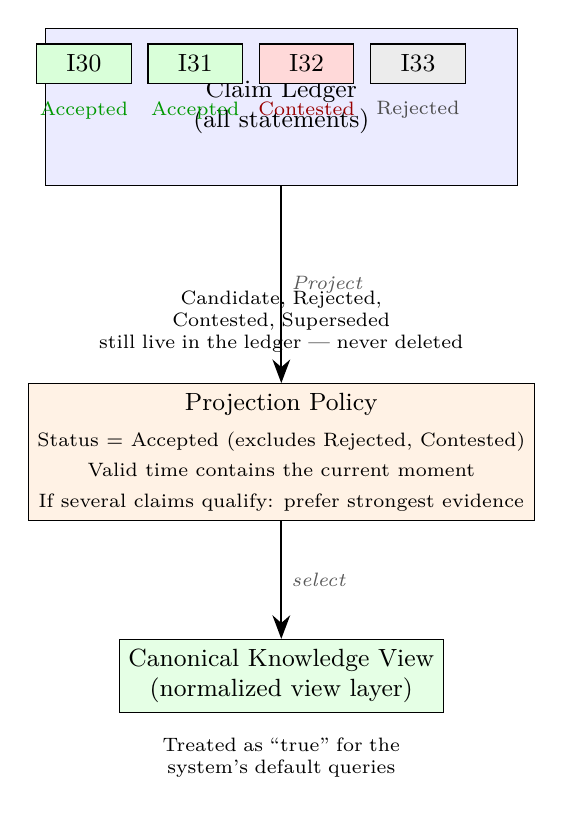
\begin{tikzpicture}[
    box/.style={rectangle, draw, minimum width=3cm, minimum height=0.8cm, align=center, font=\small},
    arrow/.style={-{Stealth[length=3mm]}, thick},
    label/.style={font=\scriptsize\itshape, text=gray!70!black},
]

% Claim Ledger (large container)
\node[box, fill=blue!8, minimum width=6cm, minimum height=2cm] (ledger) {Claim Ledger\\(all statements)};

% Individual claims inside
\node[box, fill=green!15, minimum width=1.2cm, minimum height=0.5cm, below=0.2cm of ledger.north west, xshift=0.5cm] (i30) {I30};
\node[box, fill=green!15, minimum width=1.2cm, minimum height=0.5cm, right=0.2cm of i30] (i31) {I31};
\node[box, fill=red!15, minimum width=1.2cm, minimum height=0.5cm, right=0.2cm of i31] (i32) {I32};
\node[box, fill=gray!15, minimum width=1.2cm, minimum height=0.5cm, right=0.2cm of i32] (i33) {I33};

\node[below=0.1cm of i30, font=\scriptsize, text=green!60!black] {Accepted};
\node[below=0.1cm of i31, font=\scriptsize, text=green!60!black] {Accepted};
\node[below=0.1cm of i32, font=\scriptsize, text=red!60!black] {Contested};
\node[below=0.1cm of i33, font=\scriptsize, text=gray!60!black] {Rejected};

\node[below=1.2cm of ledger, font=\scriptsize, align=center, text width=5cm] {Candidate, Rejected, Contested, Superseded\\still live in the ledger --- never deleted};

% Projection policy
\node[box, fill=orange!10, below=2.5cm of ledger, minimum width=4cm] (policy) {Projection Policy\\[2pt]
\scriptsize Status = Accepted (excludes Rejected, Contested)\\
\scriptsize Valid time contains the current moment\\
\scriptsize If several claims qualify: prefer strongest evidence};

% Arrow from ledger to policy
\draw[arrow] (ledger.south) -- node[right, label] {Project} (policy.north);

% Canonical view
\node[box, fill=green!10, below=1.5cm of policy, minimum width=4cm] (canonical) {Canonical Knowledge View\\(normalized view layer)};
\draw[arrow] (policy.south) -- node[right, label] {select} (canonical.north);

\node[below=0.2cm of canonical, font=\scriptsize, align=center, text width=4cm] {Treated as ``true'' for the system's default queries};

\end{tikzpicture}
\end{document}
